\documentclass[11pt]{article}
\usepackage[margin=1in]{geometry}
\usepackage{amsmath,amssymb,booktabs,graphicx,setspace,caption,hyperref}
\usepackage[T1]{fontenc}
\usepackage{mathpazo}
\setlength{\parindent}{0pt}
\setlength{\parskip}{0.6em}
\captionsetup{font=small,skip=6pt}
\title{Panel MS-AR(1) on SOE log real GDP per worker}
\author{}
\date{}
\begin{document}
\maketitle
\tableofcontents
\clearpage
\section{Model}
Joint panel Markov-switching AR(1) around a trend, with three regimes:
\begin{align}
y_{it} &= \tau_{it} + z_{it}, \\
z_{i,t+1} &= \bigl(1-\rho(s_{it})\bigr)\mu(s_{it}) + \rho(s_{it})\, z_{it} + \sigma(s_{it})\,\varepsilon_{it}, \\
s_{i,t+1} &\sim \Pi(\,\cdot\mid s_{it}).
\end{align}
Here $\tau_{it}$ is a (possibly country-specific) trend in calendar time; the six specifications below differ in how $\tau_{it}$ is constructed.
Countries are independent given shared Markov parameters; latent paths $s_{it}$ are country-specific. The regime dated $t$ governs the transition from $z_t$ to $z_{t+1}$. $\sigma$ switches with the regime. Unless noted, $\rho$ is regime-specific and the median $\mu$ is pinned at 0 after ordering. The likelihood is a Hamilton filter per country, summed across the panel.
\subsection*{Trend assumptions}
\begin{enumerate}
\item Common intercept $a$ and common linear slope $g$ (joint MLE).
\item Country intercepts $a_i$ and common $g$ ($a_i$ profiled).
\item Country intercepts $a_i$ and slopes $g_i$ (both profiled).
\item Country-specific Christiano--Fitzgerald low-pass trend (cycle $=$ oscillations of 2--100 quarters / 25 years), then MS-AR on the cycle.
\item Same CF trend, with every $\mu(s)=0$.
\item Same CF trend, with one $\rho$ common to all regimes.
\end{enumerate}
Sections 4--6 are two-step: the trend is not re-estimated jointly with the cycle.
Standard errors (in parentheses) are delta-method from a numerical Hessian on shared parameters only. A dashed entry is a pinned coefficient.
\clearpage
\section{Common intercept and linear trend}
SOE sample: log real GDP per worker. 62 countries in the file, 7004 observations, 1950-Q1--2024-Q3. Fitted countries: 62. Observations: 7004. Log-likelihood: 17917.39.
Common intercept $a=-4.0009$. Common slope $g=0.0139$.
\begin{table}[h]
\centering
\caption{Regime AR(1) and transition matrix. Columns are regimes.}
\begin{tabular}{lccc}
\toprule
 & (0) & (1) & (2) \\
\midrule
$\mu$ & -0.1033 & 0.0000 & 0.7480 \\
 &  & --- &  \\ \addlinespace
$\sigma$ & 0.0099 & 0.0222 & 0.0692 \\
 & (0.0002) &  &  \\ \addlinespace
$\rho$ & 0.9900 & 0.9900 & 0.9900 \\
 &  &  &  \\ \addlinespace
$\Pi_{0\cdot}$ & 0.9754 & 0.0070 & 0.0177 \\
 & (0.0044) &  & (0.0013) \\ \addlinespace
$\Pi_{1\cdot}$ & 0.0133 & 0.9691 & 0.0176 \\
 & (0.0023) & (0.0029) & (0.0021) \\ \addlinespace
$\Pi_{2\cdot}$ & 0.0812 & 0.1445 & 0.7743 \\
 & (0.0068) & (0.0109) & (0.0112) \\ \addlinespace
\bottomrule
\end{tabular}
\end{table}
\begin{figure}[h]
\centering
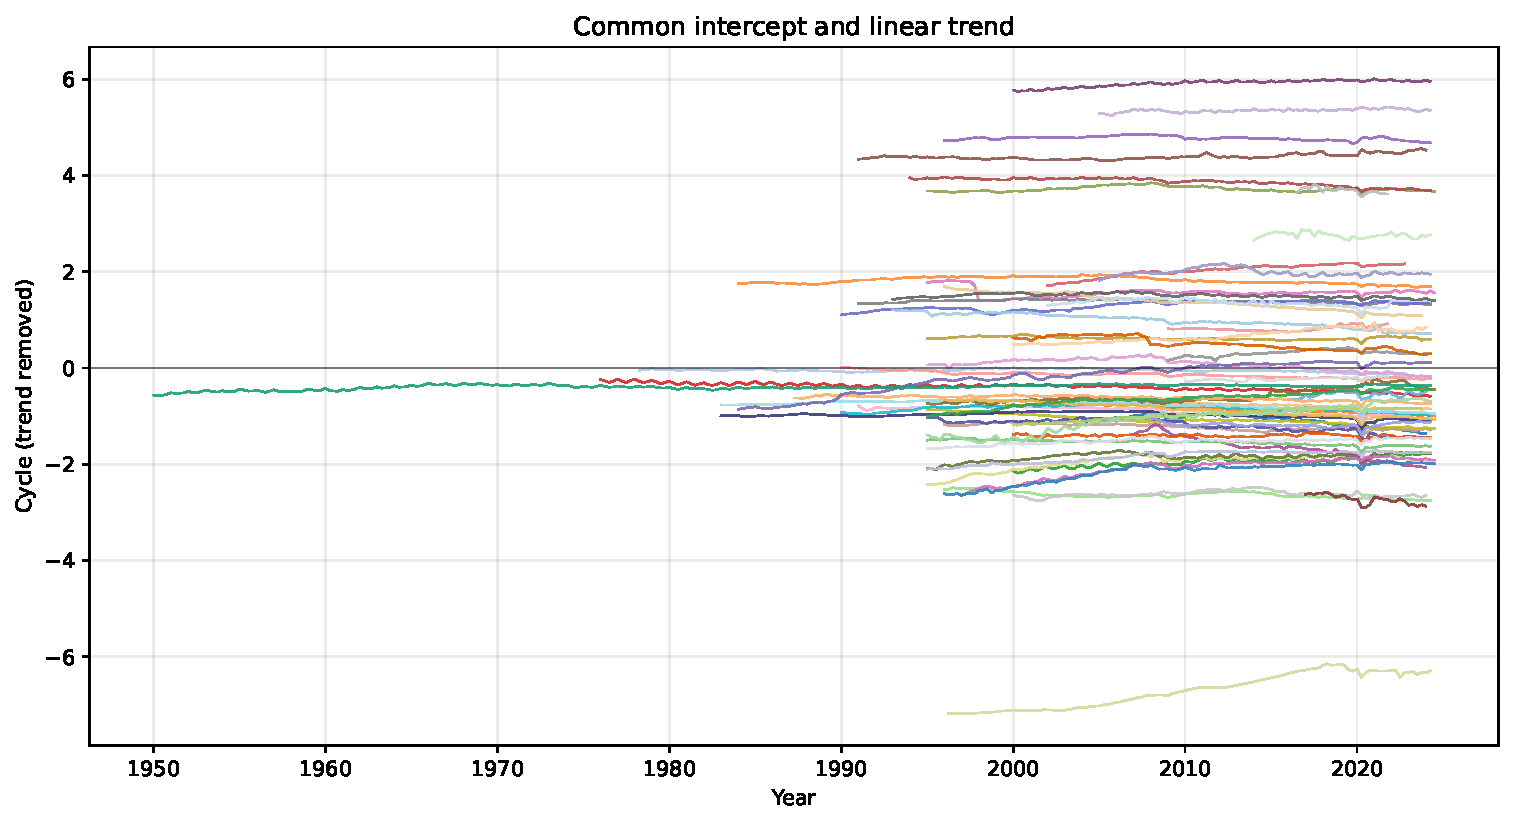
\includegraphics[width=0.75\textwidth]{figs/cycle_1_common_ag.pdf}
\caption{Country cycles after removing the section's trend.}
\end{figure}
\clearpage
\section{Country-specific intercepts, common linear trend}
SOE sample: log real GDP per worker. 62 countries in the file, 7004 observations, 1950-Q1--2024-Q3. Fitted countries: 62. Observations: 7004. Log-likelihood: 18079.16. Standard errors omitted.
Country intercepts $a_i$: mean -3.863, min -10.356, max 2.154. Common slope $g=0.0115$.
\begin{table}[h]
\centering
\caption{Regime AR(1) and transition matrix. Columns are regimes.}
\begin{tabular}{lccc}
\toprule
 & (0) & (1) & (2) \\
\midrule
$\mu$ & -0.1298 & 0.0000 & 0.2260 \\
 &  & --- &  \\ \addlinespace
$\sigma$ & 0.0218 & 0.0682 & 0.0097 \\
 &  &  &  \\ \addlinespace
$\rho$ & 0.9900 & 0.8938 & 0.9892 \\
 &  &  &  \\ \addlinespace
$\Pi_{0\cdot}$ & 0.9426 & 0.0200 & 0.0374 \\
 &  &  &  \\ \addlinespace
$\Pi_{1\cdot}$ & 0.0932 & 0.7964 & 0.1104 \\
 &  &  &  \\ \addlinespace
$\Pi_{2\cdot}$ & 0.0232 & 0.0106 & 0.9662 \\
 &  &  &  \\ \addlinespace
\bottomrule
\end{tabular}
\end{table}
\begin{figure}[h]
\centering
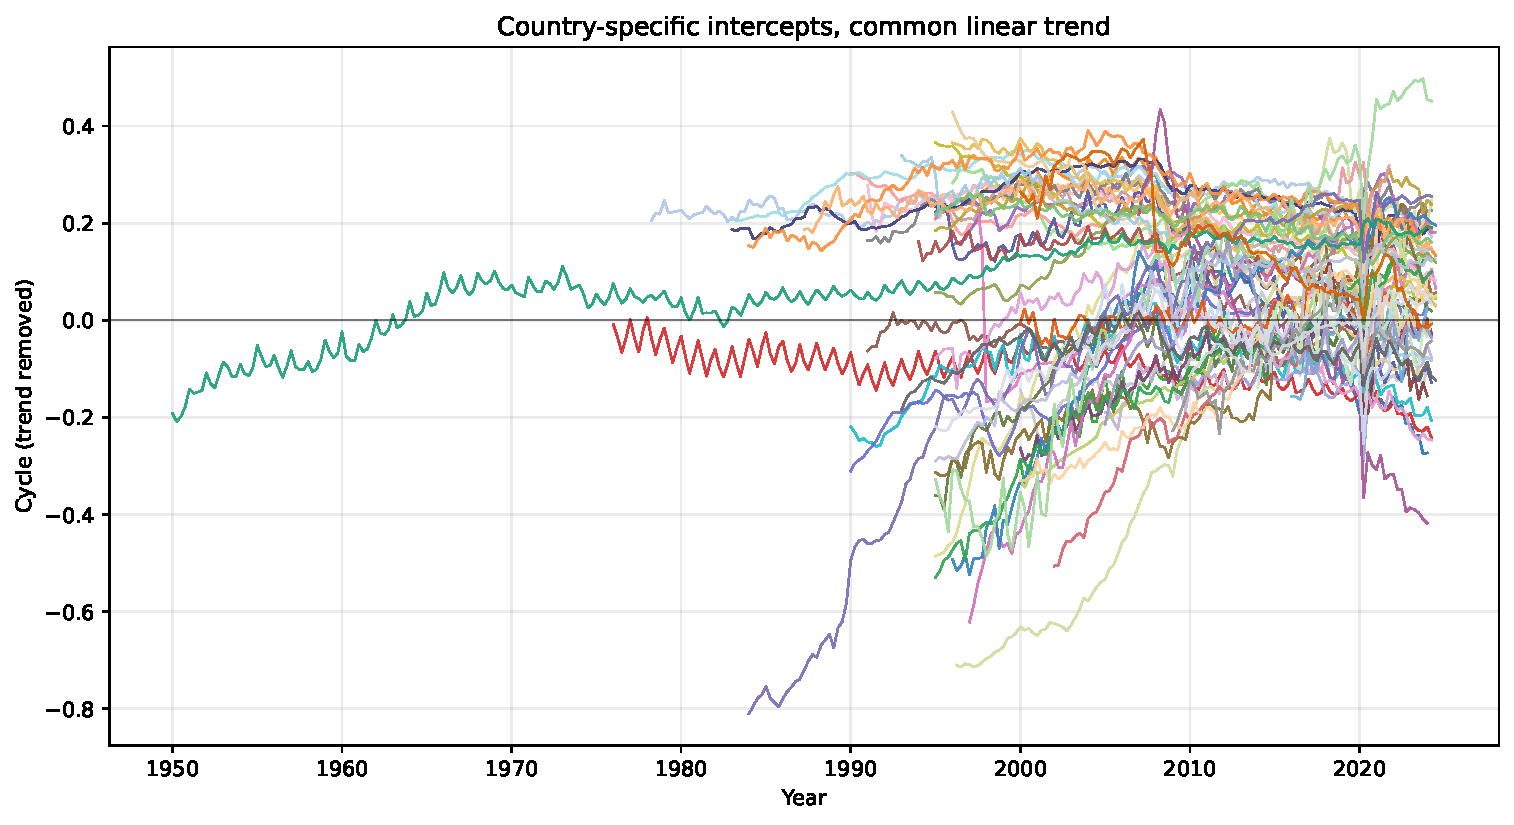
\includegraphics[width=0.75\textwidth]{figs/cycle_2_ai_common_g.pdf}
\caption{Country cycles after removing the section's trend.}
\end{figure}
\clearpage
\section{Country-specific intercepts and linear trends}
SOE sample: log real GDP per worker. 62 countries in the file, 7004 observations, 1950-Q1--2024-Q3. Fitted countries: 62. Observations: 7004. Log-likelihood: 18357.24.
Country intercepts $a_i$: mean -3.974, min -13.117, max 2.031. Country slopes $g_i$: mean 0.0140, min -0.0309, max 0.0547.
\begin{table}[h]
\centering
\caption{Regime AR(1) and transition matrix. Columns are regimes.}
\begin{tabular}{lccc}
\toprule
 & (0) & (1) & (2) \\
\midrule
$\mu$ & -0.0854 & 0.0000 & 0.0341 \\
 & (0.0344) & --- & (0.0005) \\ \addlinespace
$\sigma$ & 0.0655 & 0.0094 & 0.0211 \\
 &  &  &  \\ \addlinespace
$\rho$ & 0.8490 & 0.9751 & 0.8981 \\
 & (0.0677) & (0.0056) & (0.0098) \\ \addlinespace
$\Pi_{0\cdot}$ & 0.7770 & 0.0740 & 0.1491 \\
 & (0.0263) &  &  \\ \addlinespace
$\Pi_{1\cdot}$ & 0.0204 & 0.9717 & 0.0080 \\
 & (0.0016) & (0.0032) &  \\ \addlinespace
$\Pi_{2\cdot}$ & 0.0172 & 0.0179 & 0.9648 \\
 & (0.0043) & (0.0029) & (0.0030) \\ \addlinespace
\bottomrule
\end{tabular}
\end{table}
\begin{figure}[h]
\centering
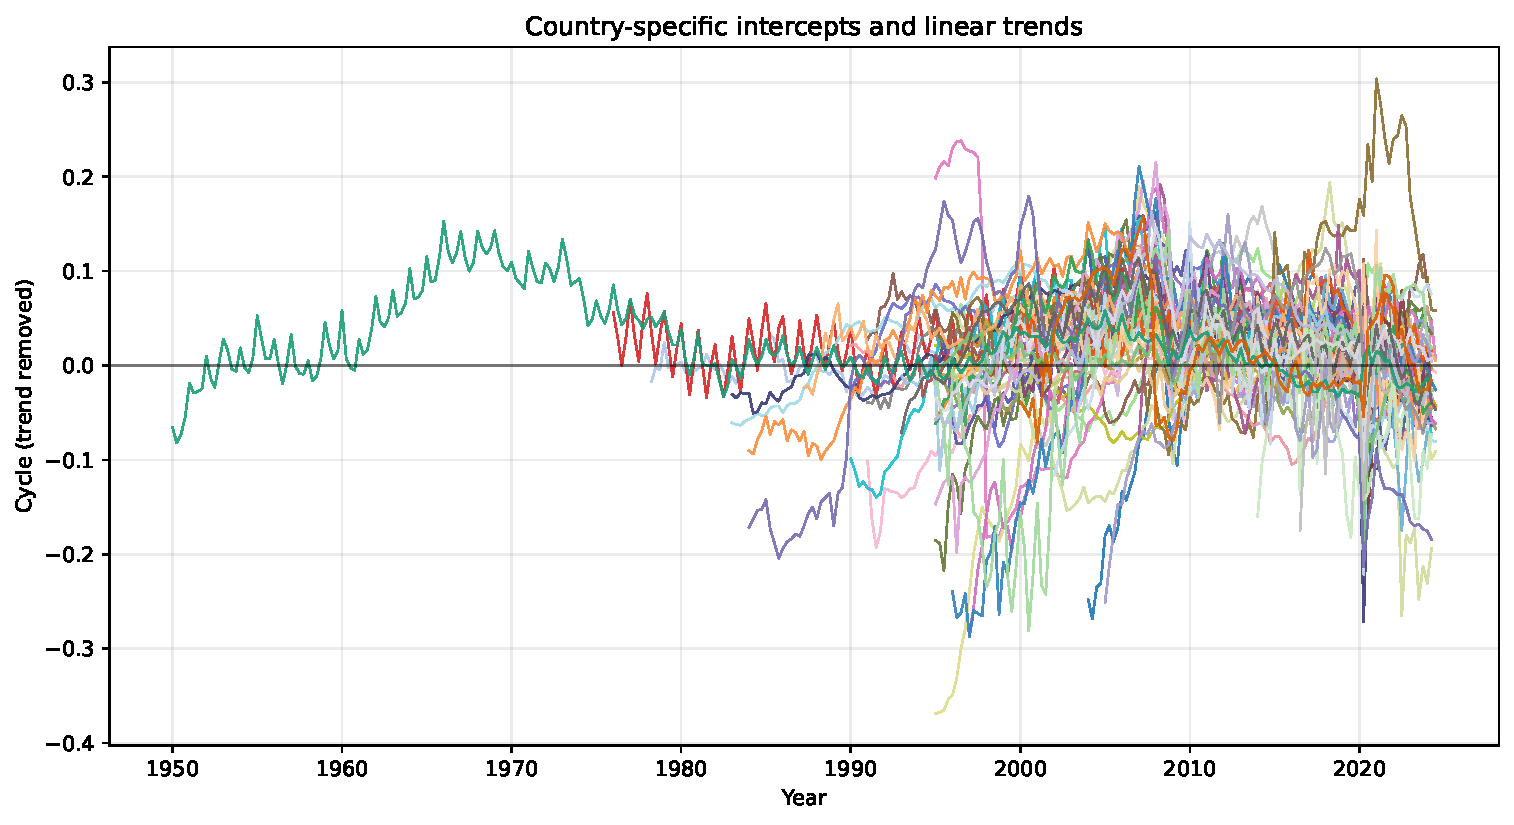
\includegraphics[width=0.75\textwidth]{figs/cycle_3_ai_gi.pdf}
\caption{Country cycles after removing the section's trend.}
\end{figure}
\clearpage
\section{Country-specific CF filtered trend (25 years)}
SOE sample: log real GDP per worker. 62 countries in the file, 7004 observations, 1950-Q1--2024-Q3. Fitted countries: 62. Observations: 7004. Log-likelihood: 18637.48.
Christiano--Fitzgerald low-pass trend: periods longer than 100 observations (25 years).
\begin{table}[h]
\centering
\caption{Regime AR(1) and transition matrix. Columns are regimes.}
\begin{tabular}{lccc}
\toprule
 & (0) & (1) & (2) \\
\midrule
$\mu$ & -0.0173 & 0.0000 & 0.0027 \\
 & (0.0054) & --- & (0.0025) \\ \addlinespace
$\sigma$ & 0.0582 & 0.0091 & 0.0204 \\
 & (0.0026) & (0.0002) & (0.0005) \\ \addlinespace
$\rho$ & 0.4857 & 0.9242 & 0.8484 \\
 & (0.0470) & (0.0072) & (0.0115) \\ \addlinespace
$\Pi_{0\cdot}$ & 0.7641 & 0.0682 & 0.1676 \\
 & (0.0317) & (0.0193) & (0.0325) \\ \addlinespace
$\Pi_{1\cdot}$ & 0.0191 & 0.9725 & 0.0085 \\
 & (0.0033) & (0.0034) & (0.0031) \\ \addlinespace
$\Pi_{2\cdot}$ & 0.0208 & 0.0164 & 0.9628 \\
 & (0.0044) & (0.0040) & (0.0055) \\ \addlinespace
\bottomrule
\end{tabular}
\end{table}
\begin{figure}[h]
\centering
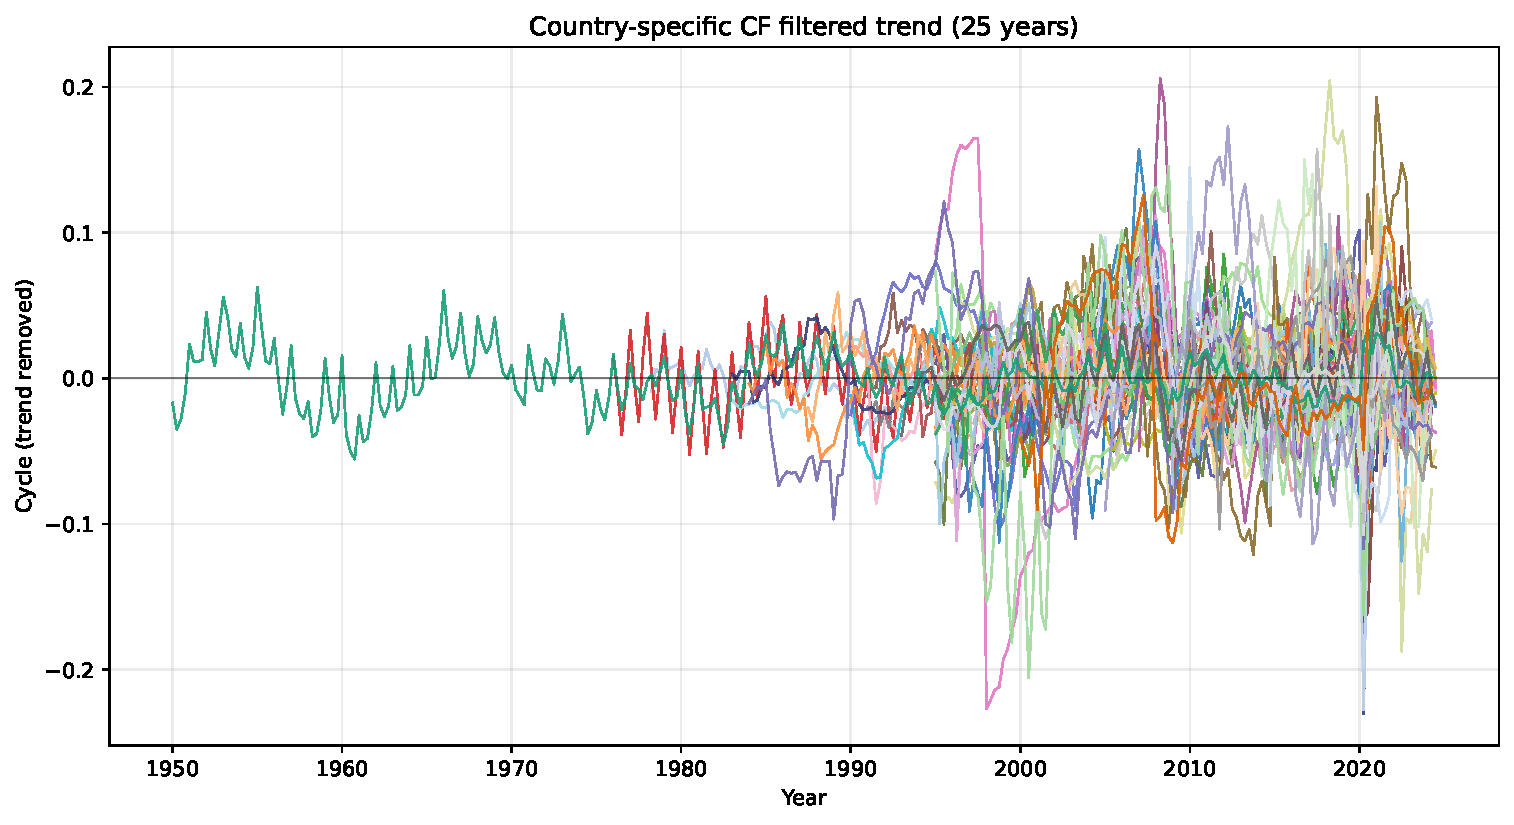
\includegraphics[width=0.75\textwidth]{figs/cycle_4_cf.pdf}
\caption{Country cycles after removing the section's trend.}
\end{figure}
\clearpage
\section{CF filtered trend, all regime means restricted to 0}
SOE sample: log real GDP per worker. 62 countries in the file, 7004 observations, 1950-Q1--2024-Q3. Fitted countries: 62. Observations: 7004. Log-likelihood: 18632.52.
Christiano--Fitzgerald low-pass trend: periods longer than 100 observations (25 years).
\begin{table}[h]
\centering
\caption{Regime AR(1) and transition matrix. Columns are regimes.}
\begin{tabular}{lccc}
\toprule
 & (0) & (1) & (2) \\
\midrule
$\mu$ & 0.0000 & 0.0000 & 0.0000 \\
 & --- & --- & --- \\ \addlinespace
$\sigma$ & 0.0091 & 0.0204 & 0.0589 \\
 & (0.0002) & (0.0005) & (0.0027) \\ \addlinespace
$\rho$ & 0.9264 & 0.8441 & 0.5308 \\
 & (0.0091) & (0.0155) & (0.0501) \\ \addlinespace
$\Pi_{0\cdot}$ & 0.9723 & 0.0082 & 0.0194 \\
 & (0.0034) & (0.0031) & (0.0034) \\ \addlinespace
$\Pi_{1\cdot}$ & 0.0165 & 0.9638 & 0.0198 \\
 & (0.0040) & (0.0055) & (0.0044) \\ \addlinespace
$\Pi_{2\cdot}$ & 0.0681 & 0.1613 & 0.7706 \\
 & (0.0191) & (0.0325) & (0.0322) \\ \addlinespace
\bottomrule
\end{tabular}
\end{table}
\begin{figure}[h]
\centering
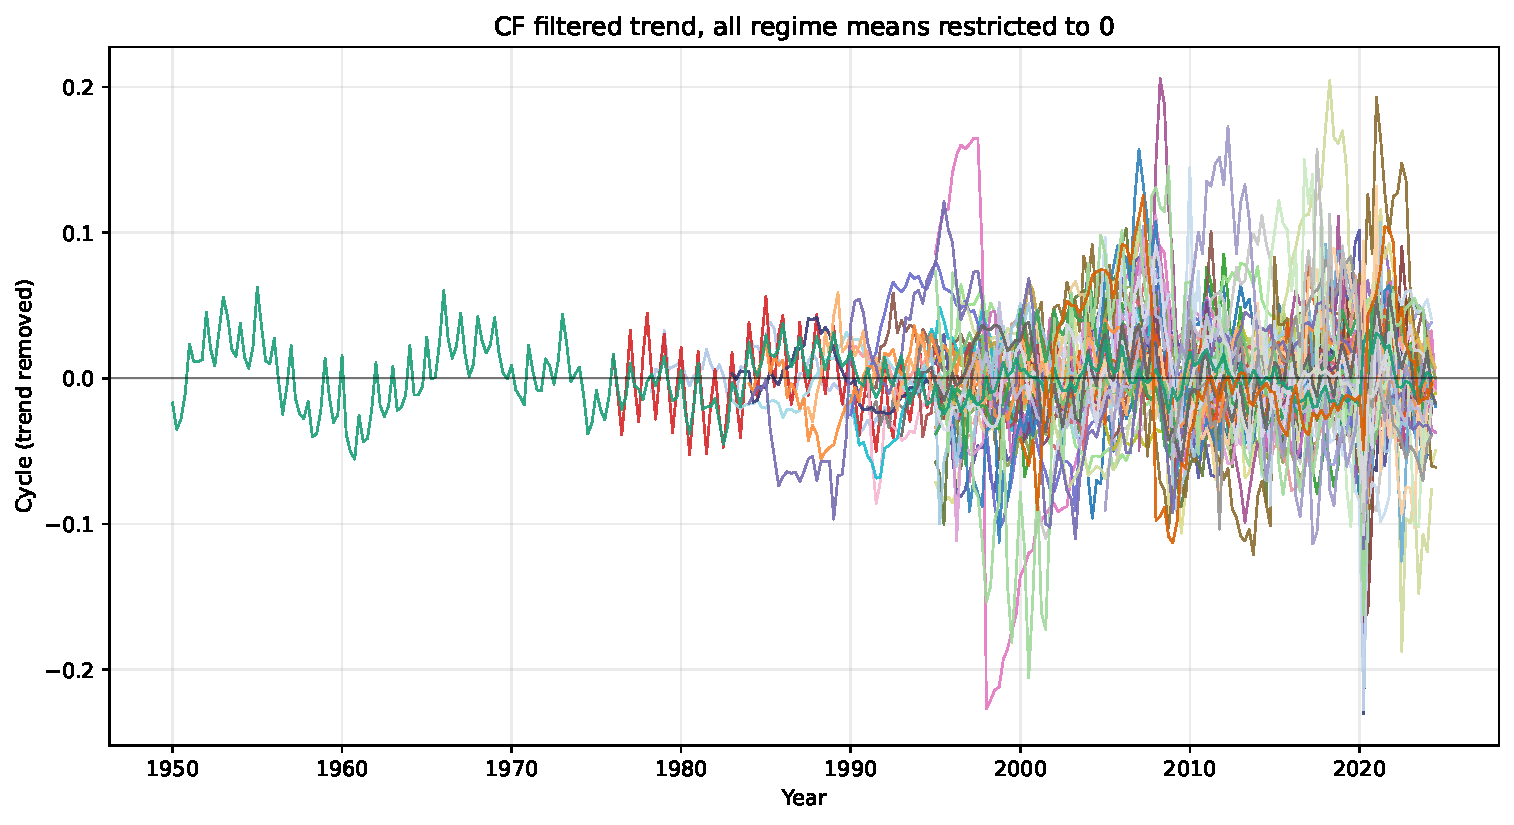
\includegraphics[width=0.75\textwidth]{figs/cycle_5_cf_zero_mu.pdf}
\caption{Country cycles after removing the section's trend.}
\end{figure}
\clearpage
\section{CF filtered trend, common $\rho$}
SOE sample: log real GDP per worker. 62 countries in the file, 7004 observations, 1950-Q1--2024-Q3. Fitted countries: 62. Observations: 7004. Log-likelihood: 18572.70.
Christiano--Fitzgerald low-pass trend: periods longer than 100 observations (25 years).
\begin{table}[h]
\centering
\caption{Regime AR(1) and transition matrix. Columns are regimes.}
\begin{tabular}{lccc}
\toprule
 & (0) & (1) & (2) \\
\midrule
$\mu$ & -0.0304 & 0.0000 & 0.0017 \\
 & (0.0246) & --- & (0.0032) \\ \addlinespace
$\sigma$ & 0.0656 & 0.0093 & 0.0208 \\
 & (0.0030) & (0.0002) & (0.0005) \\ \addlinespace
$\rho$ (common) & 0.8822 & 0.8822 & 0.8822 \\
 & (0.0061) & (0.0061) & (0.0061) \\ \addlinespace
$\Pi_{0\cdot}$ & 0.7624 & 0.0661 & 0.1715 \\
 & (0.0322) & (0.0202) & (0.0340) \\ \addlinespace
$\Pi_{1\cdot}$ & 0.0172 & 0.9742 & 0.0086 \\
 & (0.0030) & (0.0034) & (0.0032) \\ \addlinespace
$\Pi_{2\cdot}$ & 0.0191 & 0.0166 & 0.9643 \\
 & (0.0041) & (0.0041) & (0.0055) \\ \addlinespace
\bottomrule
\end{tabular}
\end{table}
\begin{figure}[h]
\centering
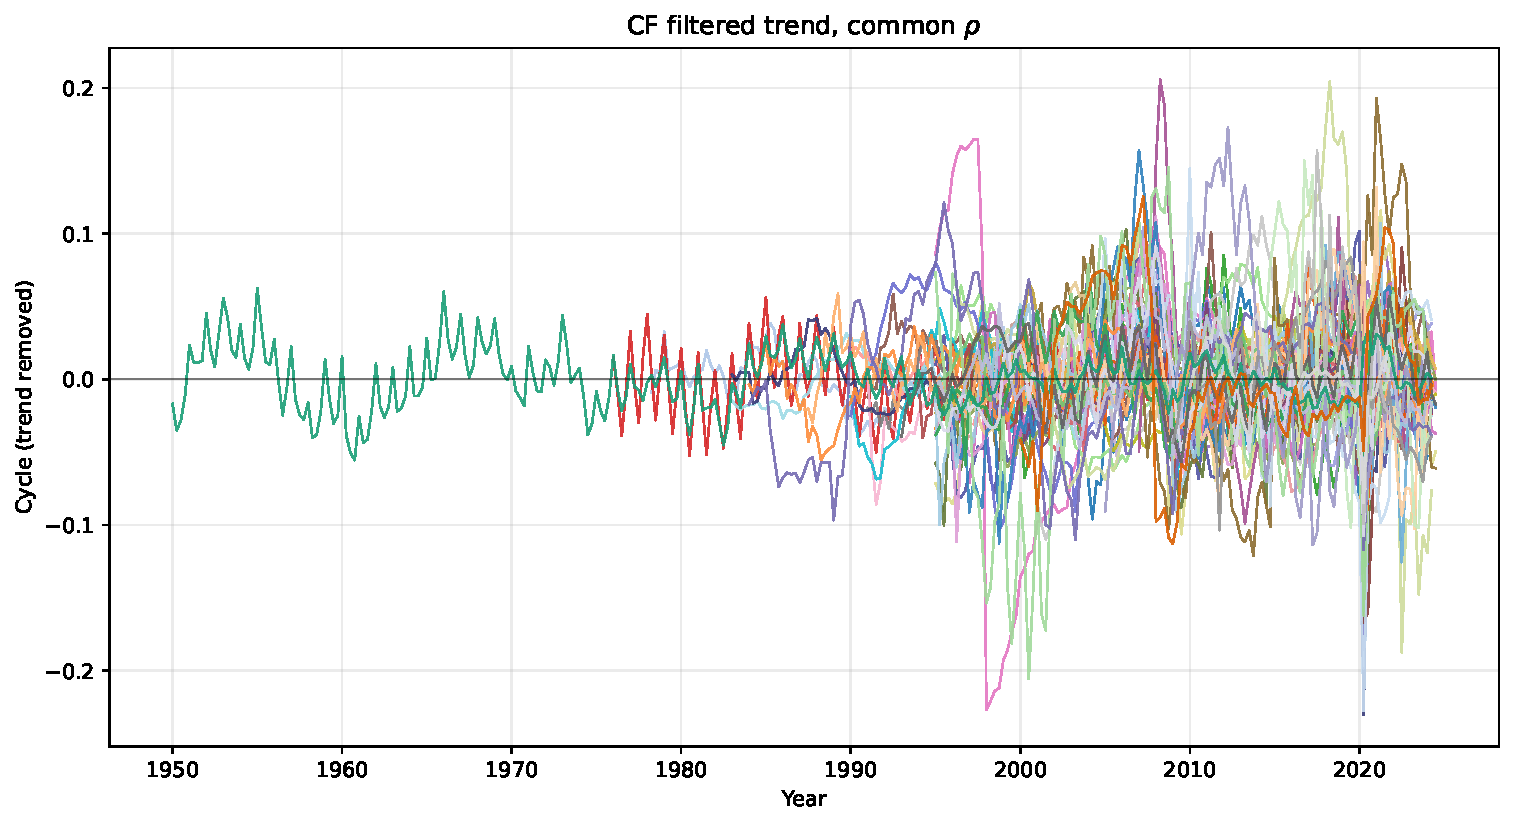
\includegraphics[width=0.75\textwidth]{figs/cycle_6_cf_common_rho.pdf}
\caption{Country cycles after removing the section's trend.}
\end{figure}
\end{document}
